\documentclass[12pt]{article}
\usepackage[a4paper, margin=2cm]{geometry}
\usepackage{amsmath}
\usepackage{array}
\usepackage{tikz}
\usepackage{tikz-feynman}
\tikzfeynmanset{compat=1.1.0}

\setlength{\parindent}{0pt}

\begin{document}

\section*{\(W^{\pm}\) Decays}

\textbf{Example:} A $W^-$ boson decays into an electron and an electron antineutrino:
\[
W^- \rightarrow e^- + \bar{\nu}_e
\]

\vspace{0.5cm}

% Two-column layout
\begin{tabular}{l l}

% LEFT COLUMN
\begin{minipage}[t]{0.46\textwidth}
\vspace{0pt}
\textbf{Feynman diagram}

\vspace{0.6cm}

\begin{tikzpicture}
\begin{feynman}
  % Vertices
  \vertex (W) at (0,2) {};
  \vertex [coordinate] (v) at (3,2) {};

  \vertex (e)  at (4,4) {\(e^-\)};
  \vertex (nu) at (5,3) {\(\bar{\nu}_e\)};

  \diagram*{
    (W) -- [boson, edge label=\(W^-\), momentum'={}] (v),
    (v) -- [fermion] (e),
    (v) -- [fermion] (nu),
  };
\end{feynman}
\end{tikzpicture}
\end{minipage}
&
% RIGHT COLUMN
\begin{minipage}[t]{0.50\textwidth}
\vspace{0pt}

\renewcommand{\arraystretch}{1.4}
\begin{tabular}{@{}l c c c c c@{}}
 & \(W^-\) & \(\Rightarrow\) & \(e^-\) & \(+\) & \(\bar{\nu}_e\) \\
Charge & $-1$ & $=$ & $-1$ & $+$ & $0$ \\
Lepton no. & $0$ & $=$ & $+1$ & $+$ & $-1$ \\
Baryon no. & $0$ & $=$ & $0$ & $+$ & $0$ \\
\end{tabular}

\vspace{0.6cm}

\textbf{Energy check}

Energy in $= 80.4\,\mathrm{GeV}$

Energy out $= 0.511\,\mathrm{MeV}$ $(e^- + \bar{\nu}_e)$

\end{minipage}

\end{tabular}

\vspace{0.9cm}

\textbf{Conclusion:} The rest mass of the products ($e^-$ and $\bar{\nu}_e$) is far less than the rest mass of the $W^-$. 
All listed conservation laws are satisfied, so this decay is allowed.

\section*{Practice: $W^-$ Decays}

%%%%%%%%%%%%%%%%%%%%%%%%%%%%%%%%%%%%%%%%%%%%
% Q1
%%%%%%%%%%%%%%%%%%%%%%%%%%%%%%%%%%%%%%%%%%%%

\textbf{Q1:} Determine the unknown particle:
\[
W^- \rightarrow \tau^- + x
\]

\vspace{0.5cm}

\begin{tabular}{l l}

% LEFT COLUMN
\begin{minipage}[t]{0.46\textwidth}
\vspace{0pt}
\textbf{Feynman diagram}

\vspace{0.6cm}

\begin{tikzpicture}
\begin{feynman}
  \vertex (W) at (0,2) {};
  \vertex [coordinate] (v) at (3,2) {};

  \vertex (tau) at (4,4) {\(\tau^-\)};
  \vertex (x)   at (5,3) {\(x\)};

  \diagram*{
    (W) -- [boson, edge label=\(W^-\), momentum'={}] (v),
    (v) -- [fermion] (tau),
    (v) -- [fermion] (x),
  };
\end{feynman}
\end{tikzpicture}
\end{minipage}
&
% RIGHT COLUMN
\begin{minipage}[t]{0.50\textwidth}
\vspace{0pt}

\renewcommand{\arraystretch}{1.4}
\begin{tabular}{@{}l c c c c c@{}}
 & \(W^-\) & \(\Rightarrow\) & \(\tau^-\) & \(+\) & \(x\) \\
Charge &  &  &  &  &  \\
Lepton no. &  &  &  &  &  \\
Baryon no. &  &  &  &  &  \\
\end{tabular}

\vspace{0.6cm}

\textbf{Energy check}

Energy in $=$

Energy out $=$

\end{minipage}

\end{tabular}

\vspace{0.5cm}

\textbf{Conclusion:}

\vspace{2.5cm}

%%%%%%%%%%%%%%%%%%%%%%%%%%%%%%%%%%%%%%%%%%%%
% Q2
%%%%%%%%%%%%%%%%%%%%%%%%%%%%%%%%%%%%%%%%%%%%
\newpage
\textbf{Q2:} Determine the unknown particle:
\[
W^- \rightarrow d + x
\]

\vspace{0.5cm}

\begin{tabular}{l l}

% LEFT COLUMN
\begin{minipage}[t]{0.46\textwidth}
\vspace{0pt}
\textbf{Feynman diagram}

\vspace{0.6cm}

\begin{tikzpicture}
\begin{feynman}
  \vertex (W) at (0,2) {};
  \vertex [coordinate] (v) at (3,2) {};

  \vertex (d) at (4,4) {\(d\)};
  \vertex (x) at (5,3) {\(x\)};

  \diagram*{
    (W) -- [boson, edge label=\(W^-\), momentum'={}] (v),
    (v) -- [fermion] (d),
    (v) -- [fermion] (x),
  };
\end{feynman}
\end{tikzpicture}
\end{minipage}
&
% RIGHT COLUMN
\begin{minipage}[t]{0.50\textwidth}
\vspace{0pt}

\renewcommand{\arraystretch}{1.4}
\begin{tabular}{@{}l c c c c c@{}}
 & \(W^-\) & \(\Rightarrow\) & \(d\) & \(+\) & \(x\) \\
Charge &  &  &  &  &  \\
Lepton no. &  &  &  &  &  \\
Baryon no. &  &  &  &  &  \\
\end{tabular}

\vspace{0.6cm}

\textbf{Energy check}

Energy in $=$

Energy out $=$

\end{minipage}

\end{tabular}

\vspace{0.5cm}

\textbf{Conclusion:}

\vspace{2.5cm}

%%%%%%%%%%%%%%%%%%%%%%%%%%%%%%%%%%%%%%%%%%%%
% Q3
%%%%%%%%%%%%%%%%%%%%%%%%%%%%%%%%%%%%%%%%%%%%

\textbf{Q3:} Determine the unknown particle:
\[
W^- \rightarrow \bar{c} + x
\]

\vspace{0.5cm}

\begin{tabular}{l l}

% LEFT COLUMN
\begin{minipage}[t]{0.46\textwidth}
\vspace{0pt}
\textbf{Feynman diagram}

\vspace{0.6cm}

\begin{tikzpicture}
\begin{feynman}
  \vertex (W) at (0,2) {};
  \vertex [coordinate] (v) at (3,2) {};

  \vertex (cbar) at (4,4) {\(\bar{c}\)};
  \vertex (x)    at (5,3) {\(x\)};

  \diagram*{
    (W) -- [boson, edge label=\(W^-\), momentum'={}] (v),
    (v) -- [fermion] (cbar),
    (v) -- [fermion] (x),
  };
\end{feynman}
\end{tikzpicture}
\end{minipage}
&
% RIGHT COLUMN
\begin{minipage}[t]{0.50\textwidth}
\vspace{0pt}

\renewcommand{\arraystretch}{1.4}
\begin{tabular}{@{}l c c c c c@{}}
 & \(W^-\) & \(\Rightarrow\) & \(\bar{c}\) & \(+\) & \(x\) \\
Charge &  &  &  &  &  \\
Lepton no. &  &  &  &  &  \\
Baryon no. &  &  &  &  &  \\
\end{tabular}

\vspace{0.6cm}

\textbf{Energy check}

Energy in $=$

Energy out $=$

\end{minipage}

\end{tabular}

\vspace{0.5cm}

\textbf{Conclusion:}

\vspace{2.5cm}

%%%%%%%%%%%%%%%%%%%%%%%%%%%%%%%%%%%%%%%%%%%%
% Q4
%%%%%%%%%%%%%%%%%%%%%%%%%%%%%%%%%%%%%%%%%%%%
\newpage
\textbf{Q4:} Determine the final lepton pair that the $W^-$ boson can decay into which has not yet featured on this sheet:
\[
W^- \rightarrow x + y
\]

\vspace{0.5cm}

\begin{tabular}{l l}

% LEFT COLUMN
\begin{minipage}[t]{0.46\textwidth}
\vspace{0pt}
\textbf{Feynman diagram}

\vspace{0.6cm}

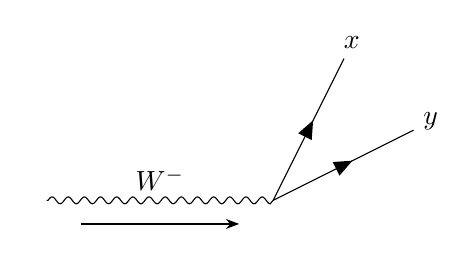
\begin{tikzpicture}
\begin{feynman}
  \vertex (W) at (0,2) {};
  \vertex [coordinate] (v) at (3,2) {};

  \vertex (x) at (4,4) {\(x\)};
  \vertex (y) at (5,3) {\(y\)};

  \diagram*{
    (W) -- [boson, edge label=\(W^-\), momentum'={}] (v),
    (v) -- [fermion] (x),
    (v) -- [fermion] (y),
  };
\end{feynman}
\end{tikzpicture}
\end{minipage}
&
% RIGHT COLUMN
\begin{minipage}[t]{0.50\textwidth}
\vspace{0pt}

\renewcommand{\arraystretch}{1.4}
\begin{tabular}{@{}l c c c c c@{}}
 & \(W^-\) & \(\Rightarrow\) & \(x\) & \(+\) & \(y\) \\
Charge &  &  &  &  &  \\
Lepton no. &  &  &  &  &  \\
Baryon no. &  &  &  &  &  \\
\end{tabular}

\vspace{0.6cm}

\textbf{Energy check}

Energy in $=$

Energy out $=$

\end{minipage}

\end{tabular}

\vspace{0.5cm}

\textbf{Conclusion:}

\vspace{2.5cm}

%%%%%%%%%%%%%%%%%%%%%%%%%%%%%%%%%%%%%%%%%%%%
% Q5
%%%%%%%%%%%%%%%%%%%%%%%%%%%%%%%%%%%%%%%%%%%%

\textbf{Q5:} Determine any other quark pair which is a valid decay of the $W^-$ boson:
\[
W^- \rightarrow x + y
\]

\vspace{0.5cm}

\begin{tabular}{l l}

% LEFT COLUMN
\begin{minipage}[t]{0.46\textwidth}
\vspace{0pt}
\textbf{Feynman diagram}

\vspace{0.6cm}

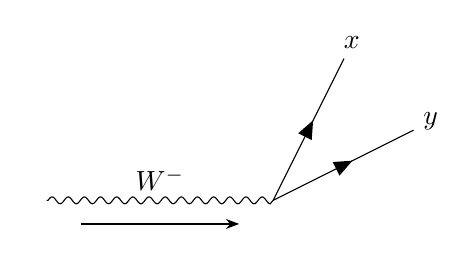
\begin{tikzpicture}
\begin{feynman}
  \vertex (W) at (0,2) {};
  \vertex [coordinate] (v) at (3,2) {};

  \vertex (x) at (4,4) {\(x\)};
  \vertex (y) at (5,3) {\(y\)};

  \diagram*{
    (W) -- [boson, edge label=\(W^-\), momentum'={}] (v),
    (v) -- [fermion] (x),
    (v) -- [fermion] (y),
  };
\end{feynman}
\end{tikzpicture}
\end{minipage}
&
% RIGHT COLUMN
\begin{minipage}[t]{0.50\textwidth}
\vspace{0pt}

\renewcommand{\arraystretch}{1.4}
\begin{tabular}{@{}l c c c c c@{}}
 & \(W^-\) & \(\Rightarrow\) & \(x\) & \(+\) & \(y\) \\
Charge &  &  &  &  &  \\
Lepton no. &  &  &  &  &  \\
Baryon no. &  &  &  &  &  \\
\end{tabular}

\vspace{0.6cm}

\textbf{Energy check}

Energy in $=$

Energy out $=$

\end{minipage}

\end{tabular}

\vspace{0.5cm}

\textbf{Conclusion:}

\vspace{2.5cm}

%%%%%%%%%%%%%%%%%%%%%%%%%%%%%%%%%%%%%%%%%%%%
% Q6
%%%%%%%%%%%%%%%%%%%%%%%%%%%%%%%%%%%%%%%%%%%%
\newpage
\textbf{Q6:} Determine a different quark pair which is a valid decay of the $W^-$ boson:
\[
W^- \rightarrow x + y
\]

\vspace{0.5cm}

\begin{tabular}{l l}

% LEFT COLUMN
\begin{minipage}[t]{0.46\textwidth}
\vspace{0pt}
\textbf{Feynman diagram}

\vspace{0.6cm}

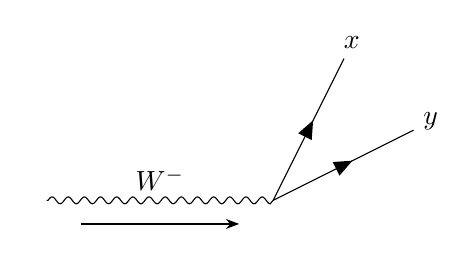
\begin{tikzpicture}
\begin{feynman}
  \vertex (W) at (0,2) {};
  \vertex [coordinate] (v) at (3,2) {};

  \vertex (x) at (4,4) {\(x\)};
  \vertex (y) at (5,3) {\(y\)};

  \diagram*{
    (W) -- [boson, edge label=\(W^-\), momentum'={}] (v),
    (v) -- [fermion] (x),
    (v) -- [fermion] (y),
  };
\end{feynman}
\end{tikzpicture}
\end{minipage}
&
% RIGHT COLUMN
\begin{minipage}[t]{0.50\textwidth}
\vspace{0pt}

\renewcommand{\arraystretch}{1.4}
\begin{tabular}{@{}l c c c c c@{}}
 & \(W^-\) & \(\Rightarrow\) & \(x\) & \(+\) & \(y\) \\
Charge &  &  &  &  &  \\
Lepton no. &  &  &  &  &  \\
Baryon no. &  &  &  &  &  \\
\end{tabular}

\vspace{0.6cm}

\textbf{Energy check}

Energy in $=$

Energy out $=$

\end{minipage}

\end{tabular}

\vspace{0.5cm}

\textbf{Conclusion:}

\vspace{2.5cm}

%%%%%%%%%%%%%%%%%%%%%%%%%%%%%%%%%%%%%%%%%%%%
% W+ Decays
%%%%%%%%%%%%%%%%%%%%%%%%%%%%%%%%%%%%%%%%%%%%

\section*{$W^+$ Decays}

%%%%%%%%%%%%%%%%%%%%%%%%%%%%%%%%%%%%%%%%%%%%
% Q7
%%%%%%%%%%%%%%%%%%%%%%%%%%%%%%%%%%%%%%%%%%%%

\textbf{Q7:} Determine the unknown particle:
\[
W^+ \rightarrow e^+ + x
\]

\vspace{0.5cm}

\begin{tabular}{l l}

% LEFT COLUMN
\begin{minipage}[t]{0.46\textwidth}
\vspace{0pt}
\textbf{Feynman diagram}

\vspace{0.6cm}

\begin{tikzpicture}
\begin{feynman}
  \vertex (W) at (0,2) {};
  \vertex [coordinate] (v) at (3,2) {};

  \vertex (ep) at (4,4) {\(e^+\)};
  \vertex (x)  at (5,3) {\(x\)};

  \diagram*{
    (W) -- [boson, edge label=\(W^+\), momentum'={}] (v),
    (v) -- [fermion] (ep),
    (v) -- [fermion] (x),
  };
\end{feynman}
\end{tikzpicture}
\end{minipage}
&
% RIGHT COLUMN
\begin{minipage}[t]{0.50\textwidth}
\vspace{0pt}

\renewcommand{\arraystretch}{1.4}
\begin{tabular}{@{}l c c c c c@{}}
 & \(W^+\) & \(\Rightarrow\) & \(e^+\) & \(+\) & \(x\) \\
Charge &  &  &  &  &  \\
Lepton no. &  &  &  &  &  \\
Baryon no. &  &  &  &  &  \\
\end{tabular}

\vspace{0.6cm}

\textbf{Energy check}

Energy in $=$

Energy out $=$

\end{minipage}

\end{tabular}

\vspace{0.5cm}

\textbf{Conclusion:}

\vspace{2.5cm}

%%%%%%%%%%%%%%%%%%%%%%%%%%%%%%%%%%%%%%%%%%%%
% Q8
%%%%%%%%%%%%%%%%%%%%%%%%%%%%%%%%%%%%%%%%%%%%
\newpage
\textbf{Q8:} Determine the unknown particle:
\[
W^+ \rightarrow u + x
\]

\vspace{0.5cm}

\begin{tabular}{l l}

% LEFT COLUMN
\begin{minipage}[t]{0.46\textwidth}
\vspace{0pt}
\textbf{Feynman diagram}

\vspace{0.6cm}

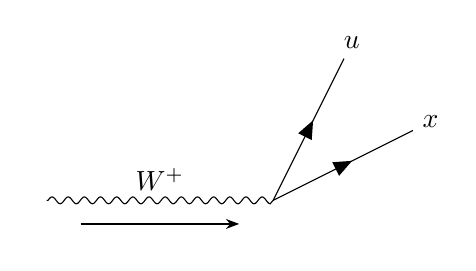
\begin{tikzpicture}
\begin{feynman}
  \vertex (W) at (0,2) {};
  \vertex [coordinate] (v) at (3,2) {};

  \vertex (u) at (4,4) {\(u\)};
  \vertex (x) at (5,3) {\(x\)};

  \diagram*{
    (W) -- [boson, edge label=\(W^+\), momentum'={}] (v),
    (v) -- [fermion] (u),
    (v) -- [fermion] (x),
  };
\end{feynman}
\end{tikzpicture}
\end{minipage}
&
% RIGHT COLUMN
\begin{minipage}[t]{0.50\textwidth}
\vspace{0pt}

\renewcommand{\arraystretch}{1.4}
\begin{tabular}{@{}l c c c c c@{}}
 & \(W^+\) & \(\Rightarrow\) & \(u\) & \(+\) & \(x\) \\
Charge &  &  &  &  &  \\
Lepton no. &  &  &  &  &  \\
Baryon no. &  &  &  &  &  \\
\end{tabular}

\vspace{0.6cm}

\textbf{Energy check}

Energy in $=$

Energy out $=$

\end{minipage}

\end{tabular}

\vspace{0.5cm}

\textbf{Conclusion:}

\vspace{2.5cm}

%%%%%%%%%%%%%%%%%%%%%%%%%%%%%%%%%%%%%%%%%%%%
% Q9
%%%%%%%%%%%%%%%%%%%%%%%%%%%%%%%%%%%%%%%%%%%%

\textbf{Q9:} Determine another lepton pair that the $W^+$ boson can decay into which has not yet featured on this sheet:
\[
W^+ \rightarrow x + y
\]

\vspace{0.5cm}

\begin{tabular}{l l}

% LEFT COLUMN
\begin{minipage}[t]{0.46\textwidth}
\vspace{0pt}
\textbf{Feynman diagram}

\vspace{0.6cm}

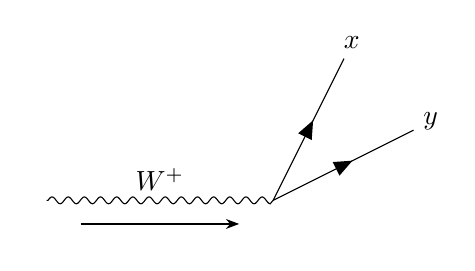
\begin{tikzpicture}
\begin{feynman}
  \vertex (W) at (0,2) {};
  \vertex [coordinate] (v) at (3,2) {};

  \vertex (x) at (4,4) {\(x\)};
  \vertex (y) at (5,3) {\(y\)};

  \diagram*{
    (W) -- [boson, edge label=\(W^+\), momentum'={}] (v),
    (v) -- [fermion] (x),
    (v) -- [fermion] (y),
  };
\end{feynman}
\end{tikzpicture}
\end{minipage}
&
% RIGHT COLUMN
\begin{minipage}[t]{0.50\textwidth}
\vspace{0pt}

\renewcommand{\arraystretch}{1.4}
\begin{tabular}{@{}l c c c c c@{}}
 & \(W^+\) & \(\Rightarrow\) & \(x\) & \(+\) & \(y\) \\
Charge &  &  &  &  &  \\
Lepton no. &  &  &  &  &  \\
Baryon no. &  &  &  &  &  \\
\end{tabular}

\vspace{0.6cm}

\textbf{Energy check}

Energy in $=$

Energy out $=$

\end{minipage}

\end{tabular}

\vspace{0.5cm}

\textbf{Conclusion:}

\vspace{2.5cm}

%%%%%%%%%%%%%%%%%%%%%%%%%%%%%%%%%%%%%%%%%%%%
% Q10
%%%%%%%%%%%%%%%%%%%%%%%%%%%%%%%%%%%%%%%%%%%%
\newpage
\textbf{Q10:} Determine the final lepton pair that the $W^+$ boson can decay into which has not yet featured on this sheet:
\[
W^+ \rightarrow x + y
\]

\vspace{0.5cm}

\begin{tabular}{l l}

% LEFT COLUMN
\begin{minipage}[t]{0.46\textwidth}
\vspace{0pt}
\textbf{Feynman diagram}

\vspace{0.6cm}

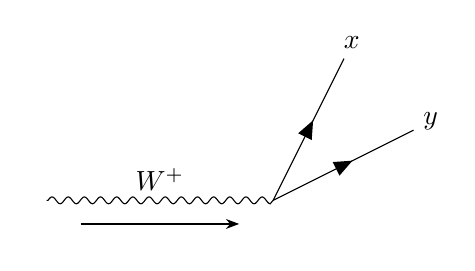
\begin{tikzpicture}
\begin{feynman}
  \vertex (W) at (0,2) {};
  \vertex [coordinate] (v) at (3,2) {};

  \vertex (x) at (4,4) {\(x\)};
  \vertex (y) at (5,3) {\(y\)};

  \diagram*{
    (W) -- [boson, edge label=\(W^+\), momentum'={}] (v),
    (v) -- [fermion] (x),
    (v) -- [fermion] (y),
  };
\end{feynman}
\end{tikzpicture}
\end{minipage}
&
% RIGHT COLUMN
\begin{minipage}[t]{0.50\textwidth}
\vspace{0pt}

\renewcommand{\arraystretch}{1.4}
\begin{tabular}{@{}l c c c c c@{}}
 & \(W^+\) & \(\Rightarrow\) & \(x\) & \(+\) & \(y\) \\
Charge &  &  &  &  &  \\
Lepton no. &  &  &  &  &  \\
Baryon no. &  &  &  &  &  \\
\end{tabular}

\vspace{0.6cm}

\textbf{Energy check}

Energy in $=$

Energy out $=$

\end{minipage}

\end{tabular}

\vspace{0.5cm}

\textbf{Conclusion:}

\vspace{2.5cm}

%%%%%%%%%%%%%%%%%%%%%%%%%%%%%%%%%%%%%%%%%%%%
% Q11
%%%%%%%%%%%%%%%%%%%%%%%%%%%%%%%%%%%%%%%%%%%%

\textbf{Q11:} Determine a valid quark pair that the $W^+$ boson can decay into:
\[
W^+ \rightarrow x + y
\]

\vspace{0.5cm}

\begin{tabular}{l l}

% LEFT COLUMN
\begin{minipage}[t]{0.46\textwidth}
\vspace{0pt}
\textbf{Feynman diagram}

\vspace{0.6cm}

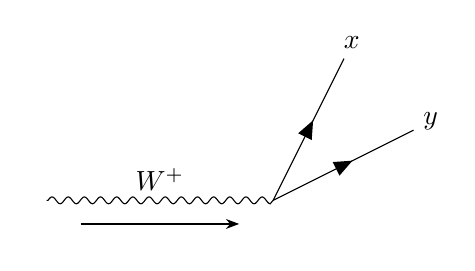
\begin{tikzpicture}
\begin{feynman}
  \vertex (W) at (0,2) {};
  \vertex [coordinate] (v) at (3,2) {};

  \vertex (x) at (4,4) {\(x\)};
  \vertex (y) at (5,3) {\(y\)};

  \diagram*{
    (W) -- [boson, edge label=\(W^+\), momentum'={}] (v),
    (v) -- [fermion] (x),
    (v) -- [fermion] (y),
  };
\end{feynman}
\end{tikzpicture}
\end{minipage}
&
% RIGHT COLUMN
\begin{minipage}[t]{0.50\textwidth}
\vspace{0pt}

\renewcommand{\arraystretch}{1.4}
\begin{tabular}{@{}l c c c c c@{}}
 & \(W^+\) & \(\Rightarrow\) & \(x\) & \(+\) & \(y\) \\
Charge &  &  &  &  &  \\
Lepton no. &  &  &  &  &  \\
Baryon no. &  &  &  &  &  \\
\end{tabular}

\vspace{0.6cm}

\textbf{Energy check}

Energy in $=$

Energy out $=$

\end{minipage}

\end{tabular}

\vspace{0.5cm}

\textbf{Conclusion:}

\vspace{2.5cm}

%%%%%%%%%%%%%%%%%%%%%%%%%%%%%%%%%%%%%%%%%%%%
% Q12
%%%%%%%%%%%%%%%%%%%%%%%%%%%%%%%%%%%%%%%%%%%%
\newpage
\textbf{Q12:} Determine a valid quark pair that the $W^+$ boson can decay into:
\[
W^+ \rightarrow x + y
\]

\vspace{0.5cm}

\begin{tabular}{l l}

% LEFT COLUMN
\begin{minipage}[t]{0.46\textwidth}
\vspace{0pt}
\textbf{Feynman diagram}

\vspace{0.6cm}

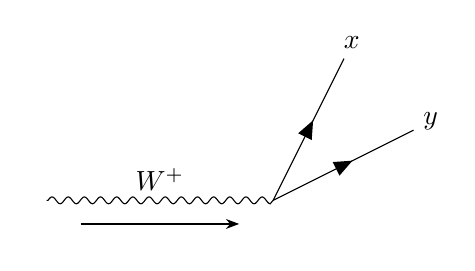
\begin{tikzpicture}
\begin{feynman}
  \vertex (W) at (0,2) {};
  \vertex [coordinate] (v) at (3,2) {};

  \vertex (x) at (4,4) {\(x\)};
  \vertex (y) at (5,3) {\(y\)};

  \diagram*{
    (W) -- [boson, edge label=\(W^+\), momentum'={}] (v),
    (v) -- [fermion] (x),
    (v) -- [fermion] (y),
  };
\end{feynman}
\end{tikzpicture}
\end{minipage}
&
% RIGHT COLUMN
\begin{minipage}[t]{0.50\textwidth}
\vspace{0pt}

\renewcommand{\arraystretch}{1.4}
\begin{tabular}{@{}l c c c c c@{}}
 & \(W^+\) & \(\Rightarrow\) & \(x\) & \(+\) & \(y\) \\
Charge &  &  &  &  &  \\
Lepton no. &  &  &  &  &  \\
Baryon no. &  &  &  &  &  \\
\end{tabular}

\vspace{0.6cm}

\textbf{Energy check}

Energy in $=$

Energy out $=$

\end{minipage}

\end{tabular}

\vspace{0.5cm}

\textbf{Conclusion:}

\vspace{2.5cm}


\end{document}